\chapter{Desenvolupament}
\section{Placa base CC1352R1}
Per analitzar el protocol BLE i veure les seves característiques s'ha utilitzat el kit per desenvolupament ràpid del microcontrolador CC1352R1.
\begin{figure}[h!]
	\begin{center}
		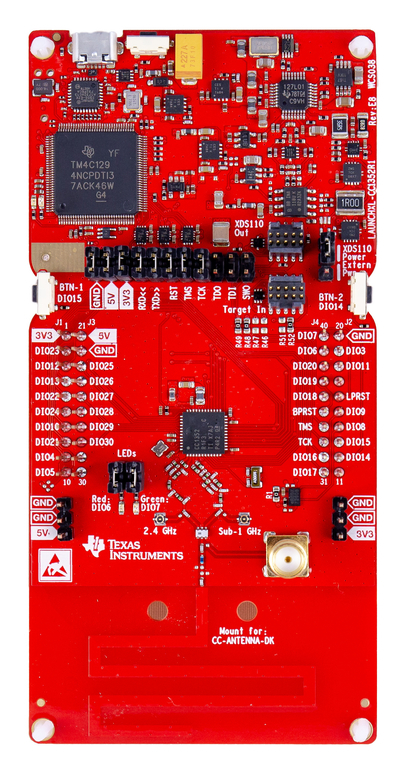
\includegraphics[width=0.5\textwidth]{./images/launchxl-cc1352r1.jpg}
		\caption{Placa \cite{placa}}
	\end{center}
\end{figure}

Aquesta placa permet el desenvolupament d'aplicacions en BLE utilitzant el microcontrolador CC1352 de Texas Instruments a continuació es descriuen les seves característiques principals \cite{placa_datasheet}.

El dispositiu CC1352R és multiprotocol i multibanda orientat a 2.4 GHz o sub-1GHz que serveix per a Thread, Zigbee, Bluetooth 5 Low Energy, IEEE 802.15.4g i 6LoWPAN. Pel que fa a memòria té 352 KB flash programable, 256 KB de ROM per a protocols i llibreries, 8 KB de Cache SRAM i 80 KB de RAM protegida amb paritat.
Pel que fa als perifèrics el més important és el ADC de 12 bits i 8 canals amb freqüència de mostreig de 200 Kmostres/s (multiplexat). També té Rellotge de Temps Real (RTC), acceleradors de operacions criptogràfiques i generador de números aleatoris.
La radio multibanda que té te un receptor amb sensibilitat de -121 dBm per a sub-1GHz i de -110 dBm a 50 Kbps o -105 dBm a 125 Kbps. El transmissor pot transmetre fins a 14 dBm sub-1GHz i 5dBm a 2.4 GHz.


\section{Software}
Per al desenvolupament de projectes per a la placa s'ha utilitzat el entorn de desenvolupament Code Composer Studio 9. El software és el SimpleLink\texttrademark\ CC13X2 versió 2.30.00.45\footnote{La versió utilitzada no és més nova per a que sigui compatible amb la revisió C del xip que s'està utilitzant.}.

\section{Project 0}
El Project 0 és el projecte instal·lat amb que les plaques vénen de fàbrica. Aquest projecte exposa certs serveis a través de BLE i et permet veure una comunicació simple entre la placa i un dispositiu mòbil.
La comunicació es fa a través del control dels dos LEDs que te la placa (els LEDs que estan directament controlats pel microcontrolador) i també per l'estat dels botons que hi ha a ambdós costats de la placa.
*Aquest projecte també inclou altres serveis en que no entrarem.

Aquest projecte serveix per tenir un bon exemple de com està dissenyada l'arquitectura dels serveis amb les seves característiques amb una relativa simple funcionalitat. A continuació s'analitzaran diferents parts dels atributs.

\subsection{Serveis de Botons i LEDs}

En la següent taula es poden veure tots els valors que hi ha tal i com estan en la taula d'atributs del servidor GATT.
Per facilitar la visualització de les dades s'han tret els zeros finals dels UUIDs propis però cal recordar que en total tenen 16 parells (128 bits en representació hexadecimal) i no només els 9 parells que surten a la taula.

\begin{center}
	\begin{table}[h!]
		\csvautotabular{data_files/projectzeroUUID.csv}
	\end{table}
\end{center}

Per poder entendre els atributs, al tenir UUID propis és necessari tenir en compte la documentació amb la que s'ha desenvolupat aquest projecte.

\begin{figure}[h!]
	\begin{center}
		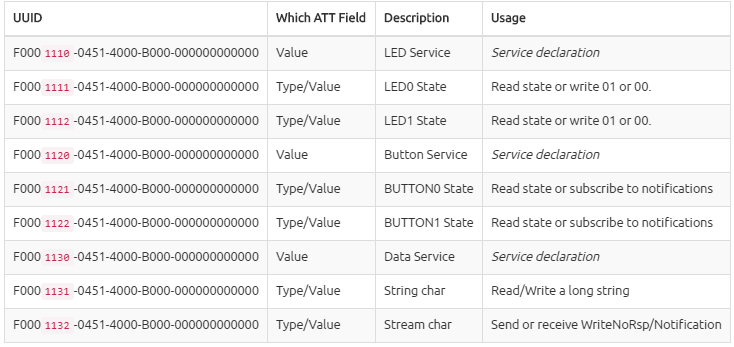
\includegraphics[width=\textwidth]{./images/Project_0_UUID.png}
		\caption{Definició dels UUIDs}
	\end{center}
	\label{project0_table}
\end{figure}

El primer que cal tenir clar és que en taula \ref{project0_table} els valors estan representats amb l'ordre en que es reben i en general els serveis estandarditzats (i també aquest servei propi) utilitza \textit{little-endian} per enviar la informació.
Això resulta en que els caràcters hexadecimals queden (per parelles) ordenats al revés.

Al analitzar els atributs es pot veure com aquells que tenen el UUID 0x2800 en el seu valor només tenen un UUID corresponent al les definicions de serveis de LEDs i de botons.
Seguidament, als atribut amb UUID 0x2803 hi ha les definicions de les característiques, en el seu valor hi ha múltiples parts.
El primer parell hexadecimal correspon a les propietats. Just després hi ha dos parells hexadecimals que identifiquen el \textit{Handle} del atribut on hi ha la característica.
I per últim la resta de caràcters corresponen al UUID que identifica la característica.

\subsection{Propietats}
\label{sec:properties}
Les propietats d'accés són un valor que identifica quines operacions i procediments es poden fer sobre la característica.
El camp té 8 bits per defecte i cada un d'ells identifica una operació o procediment.
Es poden combinar qualsevol quantitat d'aquests bits per habilitar múltiples opcions.

\begin{table}
	\begin{center}
		\begin{tabular}{|c|c|l|}
			\hline
			Binary	&	Hex		&	Property	\\	\hline
			0000 0001	&	0x01	&	Broadcast\\	\hline
			0000 0010	&	0x02	&	Read	\\	\hline
			0000 0100	&	0x04	&	Write w/o Response	\\	\hline
			0000 1000	&	0x08	&	Write	\\	\hline
			0001 0000	&	0x10	&	Notification w/o ACK	\\	\hline
			0010 0000	&	0x20	&	Indication with ACK	\\	\hline
			0100 0000	&	0x40	&	Signed Writes	\\	\hline
			1000 0000	&	0x80	&	Aditional Properties	\\	\hline
		\end{tabular}
	\end{center}
\caption{Valors de les propietats}
\end{table}


Primer de tot cal destacar la implementació de comunicacions amb o sense reconeixement. D'aquesta manera si preferim reduir la quantitat de missatges per estalviar bateria enlloc d'assegurar-se que s'ha rebut la informació es dona la opció.

Pel que fa les propietats en el Project 0 les característiques dels LEDs tenen el valor 0x0E que resulta en 0000 1110 per tant, es permet: llegir, escriure i escriure sense resposta.
En canvi les característiques del servei de botons té el valor 0x12 que suposa 0001 0010, per tant, es permet notificació sense reconeixement.

La notificació i indicació són funcions que ajuden a reduir el consum de recursos.
Quan volem saber en quin estat estan els botons de la placa contínuament es podria anar llegint el estat de la característica constantment però això suposarien molts missatges i reduiria el temps que els dispositius es poden adormir i així ser més eficients.
Per evitar aquest cas es pot configurar la característica tal que sigui la mateixa placa qui enviï el missatge automàticament quant el estat de la característica canviï.
D'aquesta manera el receptor només cal que escolti els missatges de la placa per tal de saber en quin estat està el botó.

En cas de que es vulgui indicació amb reconeixements és possible configurar-ho d'aquesta manera a través del atribut Configuració de Característica del Client identificat amb el UUID 0x2902 i estandarditzat en la especificació de Bluetooth.
Si el valor és 0 no hi ha transmissions, si el valor és 1 s'envien notificacions (sense reconeixement) i si el valor és 2 s'envien indicacions (notificacions amb reconeixement). 

El bit d'extensió de propietats, en cas que sigui 1 indica que existeix un atribut: Descriptor Propietats Esteses de Característica.
Aquest atribut te el UUID 0x2900 i el que permet és afegir més propietats de les que poden existir amb el espai limitat de 8 bits que hi ha per defecte.
Aquest sistema permet afegir fins a 16 bits més per indicar propietats, actualment estan els dos primers definits segons el estàndard i la resta estan reservats per a ús futur \cite{extended properties}.

Aquests 2 primers que estan definits són escriptura fiable i escriptura auxiliar.
L'escriptura fiable permet escriure valors amb un procediment diferent al habitual que permet assegurar-se que el valor que es vol modificar s'ha escrit i no hi han hagut errors.
Pel que fa  al'escriptura auxiliar permet escriptura al descriptor de característica [posar exemple].



\section{Client BLE}
Per poder interactuar amb un servidor de BLE és necessari tenir una implementació de client.
Com que els mòbils intel·ligents tots tenen BLE hi ha moltes aplicacions que permeten visualitzar els serveis amb les seves corresponents característiques.
També interactuar, escrivint o llegint aquells valors en que es pot.
Tot i així, no totes les aplicacions permeten rebre notificacions o utilitzar seguretat.
I les aplicacions no permeten interactuar directament amb el controlador (a través de HCI), per exemple, no poden canviar la potència de transmissió. 

Per poder tenir un control total del sistema el kit de desenvolupament que proporciona Texas Instruments conté l'aplicació BTool.
S'utilitza conjuntament amb el projecte Host Test del mateix kit per convertir la placa en un client BLE.
El projecte Host Test permet controlar les diferents capes de la pila BLE del xip a través de la interfície sèrie.
Totes les possibles peticions, tant del servidor GAP com els missatges HCI.

\subsection{Btool}
L'aplicació BTool utilitza l'API del projecte Host Test per executar les crides a les diferents capes BLE.
Primer de tot, BTool necessita saber per quina interfície ha d'interactuar amb la placa.
Al administrador de dispositius de Windows es poden trobar els ports utilitzats per la placa i els paràmetres de la conexió els indica Texas Instruments\cite{serial_params}.
Un cop s'inicia la comunicació entre BTool i la placa es pot escanejar, iniciar connexió i descobrir la taula d'atributs del servidor.
En tot moment es poden veure tots els paquets que s'envien per la interfície amb la seva corresponent interpretació en la consola.
Com que en aquesta consola apareixen tots els esdeveniments de BLE 5, permet veure quan es reben notificacions.
Un cop s'ha establert la connexió es pot interactuar amb la taula d'atributs directament.


\section{Crear un Perfil propietari}

Per poder implementar una xarxa de sensors amb BLE serà necessari disenyar un esquema pròpi en el servidor GATT.
Tal i com s'ha comentat anteriorment el servidor GATT està format per perfils que alhora agrupen serveis.
Aquests serveis son els que contenen les característiques amb les que s'interacturarà per intercanviar informació.
A continuació s'explicarà com es poden implementar perfils en l'entorn de Texas Instruments BLE Stack.

\subsection{Generar Fitxers}
Texas Instruments proporciona un Generador de Fitxers \cite{Service_Generator} que evita haver de començar de zero.
En aquesta eina s'han de definir el nom del servei, els noms de les característiques amb la seva longitud i les propietats i els corresponents UUIDs.
Aquesta eina està pensada per a ser utilitzada junt amb el Project Zero, per tant, aquest serà el projecte base per al meu cas.
Un cop s'han generat els fitxers cal copiar-los dins de Application/services en el projecte.

A parts dels fitxers generats (font i capçalera\footnote{Els fitxers de capçalera en C s'identifiquen per l'extensió .h i contenen les declaracions de funcions que es poden compartir entre múltiples fitxers font}) també cal que l'aplicació cridi a la funció que incialitza el servei registrant-los al GATT.
Aquesta és la funció [Perfil]\_AddService(..) que cal afegir dins la funció ProjectZero\_init() en la secció Inicialitació de Serveis.

Tot i que aquest generador de fitxers és molt útil alhora de tenir una estructura bàsica del projecte cal analitzar les parts importants per entendre com funciona per dins i quina relació te cada part amb BLE.

\subsection{title}

Definir UUIDs/Logitud del valor
Tal i com s'ha comentat anteriorment els UUIDs poden tenir diferents longituds depenent si corresponen a un estàndard o si son propietaris.
Quedaran definits al fitxer capçalera.

Taula de atributs
La taula d'atributs està formada per un llistat d'atributs, la estructura d'aquest ve definida en el gatt.h i s'anomena gattAttribute\_t.
Inclou el tipus d'UUID (de 16 o 128 bits), els permisos, el handle (cal deixar-lo a 0 ja que s'assigna internament pel servidor) i el valor (longitud màxima 512 bytes).

Quan sindiquen les propietats dels atributs que corresponen s'utilitzar l'operador OR (en C correspon al símbol |).
El fitxer gatt.h s'inclou dins del fitxer font i conté les definicions de tots els possibles permisos amb els seus valors en bits corresponents.

Descriptors


Callbacks (get/set write/read)
En cada servei hi ha quatre funcions de \textit{callback}.
Les funcions get i set s'utilitzen per llegir o modificar els valors que s'exposen a través de BLE.
Quant en algun punt del codi és necessari interactuar amb aquests valors es farà amb aquestes funcions.
Com que s'està treballant amb C és important posar comprovacions quant es modifiquen els valors per tal d'evitar problemes com el desbordament de memòria intermèdia\footnote{En anglès Buffer Overflow} que poden ocórrer si s'escriuen valors no vàlids.

Les funcions write i read són les que s'utilitzen per interceptar les peticions de lectura i escriptura del servidor GATT.

En aquestes funcions cal identificar en cada cas a quin atribut o valor s'esta modificant i després de comprovacions o altres funcionalitats es copia la memòria entre els arguments.

Butons
La placa que s'esta utilitzant té dos butons que s'utilitzen com a entrades de senyals.
En el fitxer principal project\_zero.c hi ha la funció ProjectZero\_handleButtonPress() que es crida quan es pressiona o es deixa de pressionar qualsevol dels botons.

Notificacions
Les notificacions serveixen per indicar al client que un valor ha canviat en el servidor.
Per poder utilitzar-les primer cal crear un CCCD
CCCD


Temporitzadors
Tal i com s'ha comentat anteriorment la placa que s'està utilitzant inclou rellotges.
Xips...
El entorn ja ens dona directament classes amb les que pot treballar amb els rellotges així facilitant el seu ús.

%Generador flux aleatori (perlin noise?)
%Per a poder fer una simulació de com funciona BLE al transmetre les mesures mediambientals i biològiques és necessari tenir alguna font d'aquesta informació.
%Les dades es generaran aleatoriament i per tant cal entendre com s'han de generar les senyals simulades en l'entorn de desenvolupament.



